\chapter{Pendahuluan}
\label{chap:pendahuluan}

\section{Latar Belakang}
\label{sec:latar_belakang}

Student Portal UNPAR\cite{studentportalunpar} merupakan sistem informasi berbasis \textit{web} yang digunakan oleh mahasiswa Universitas Katolik Parahyangan. Fitur-fitur yang dimiliki Student Portal UNPAR yaitu rencana studi, jadwal, nilai dan indeks prestasi, dan pembayaran uang kuliah. Namun, fitur-fitur tersebut masih belum cukup untuk mendukung kebutuhan akademik mahasiswa Program Studi Teknik Informatika. 

Salah satu fitur yang diperlukan oleh mahasiswa Teknik Informatika UNPAR adalah prasyarat mata kuliah. Dalam Teknik Informatika UNPAR, terdapat beberapa mata kuliah yang membutuhkan prasyarat baik prasyarat tempuh maupun prasyarat lulus. Student Portal UNPAR sudah menyediakan fitur prasyarat mata kuliah namun kurang mendukung karena data yang ditampilkan kurang akurat. Misalnya dalam pengambilan mata kuliah "`AIF453 Kecerdasan Bisnis"' membutuhkan prasyarat lulus mata kuliah "`AIF204 Manajemen Informasi dan Basis Data"' atau lulus mata kuliah "`AIF102 Algoritma dan Struktur Data"' dengan IPK di atas 2.75 (Gambar \ref{fig:1_prasyarat_tinyurl}). Namun dalam Student Portal UNPAR, prasyarat yang dicantumkan hanya lulus mata kuliah "`AIF204 Manajemen Informasi dan Basis Data"' (Gambar \ref{fig:1_prasyarat_student_portal}). Selain itu, pemeriksaan prasyarat mata kuliah tidak dilakukan secara otomatis sehingga setiap pengambilan mata kuliah tetap dianggap valid meskipun belum memenuhi prasyarat.

jsoup\cite{jsoup} merupakan \textit{library} Java yang digunakan untuk menelusuri suatu situs \textit{web} untuk mendapatkan suatu informasi. Informasi yang didapat berupa HTML yang kemudian diekstrak dan disajikan dalam bentuk \textit{Document Object Model}. Play Framework\cite{Leroux:2014} merupakan sebuah \textit{web framework} berbasis Java dan Scala. Play juga menggunakan \textit{design pattern} \textit{Model-View-Controller} (MVC) di mana \textit{model} dan \textit{controller} menggunakan bahasa Java sedangkan \textit{view} menggunakan bahasa Scala dan HTML. SIA Models\cite{siamodels} merupakan kelas-kelas dalam bahasa Java yang merepresentasikan Sistem Informasi Akademik UNPAR. Aplikasi akan dibuat dengan menggunakan Play Framework dan jsoup karena aplikasi didukung oleh SIA Models yang tersedia dalam bahasa Java. 

\begin{figure}[H]
	\centering
	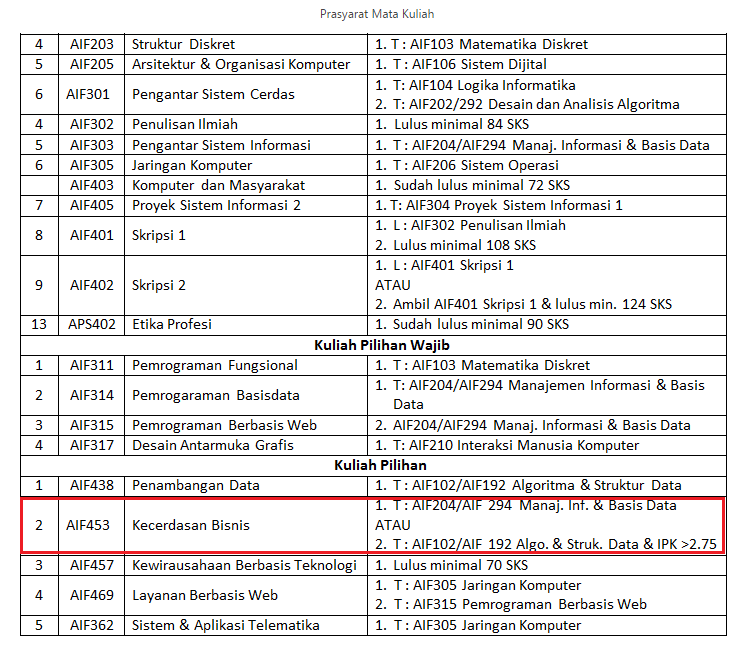
\includegraphics[scale=0.5]{Gambar/contoh-tinyurl}
	\caption{Prasyarat Mata Kuliah\cite{prasyaratIT}}
	\label{fig:1_prasyarat_tinyurl}
\end{figure}

\begin{figure}[H]
	\centering
	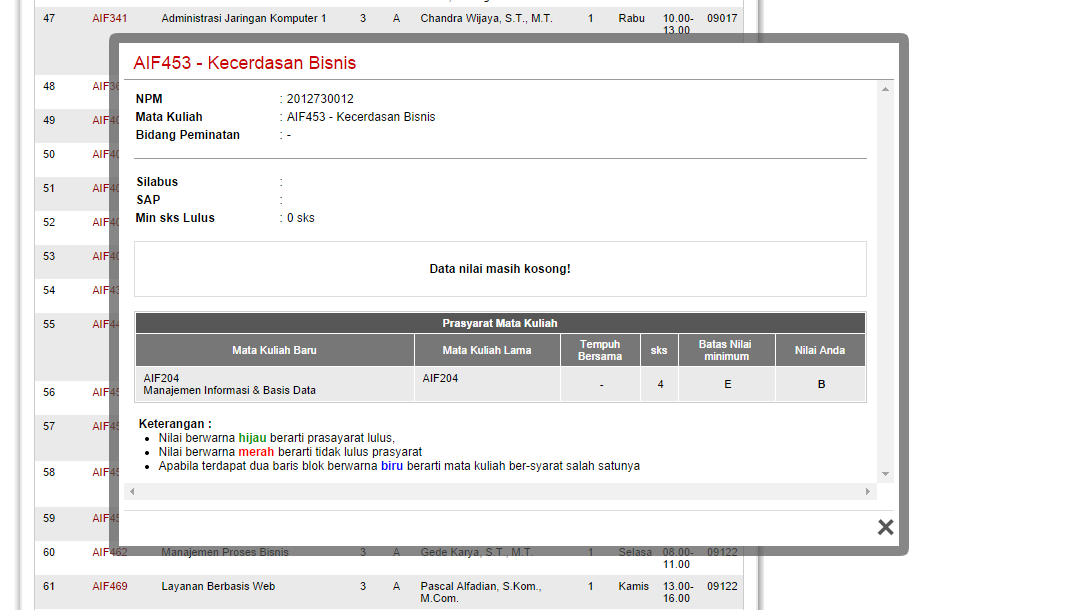
\includegraphics[scale=0.5]{Gambar/contoh-portal}
	\caption{Prasyarat Mata Kuliah Student Portal UNPAR\cite{studentportalunpar}}
	\label{fig:1_prasyarat_student_portal}
\end{figure}

Untuk mendukung kebutuhan akademik mahasiswa Program Studi Teknik Informatika, fitur-fitur yang diperlukan akan dianalisa kemudian diimplementasikan ke dalam program IT Student Portal. Program yang akan dibuat merupakan program berbasis \textit{web} menggunakan Play Framework. Selain itu, data-data yang akan ditampilkan diambil langsung dari Student Portal UNPAR dengan \textit{web scraping} menggunakan \textit{library} jsoup. Untuk melakukan pengambilan data, jsoup harus mengetahui cara kerja dari Student Portal UNPAR. Analisis komunikasi Student Portal UNPAR akan dilakukan dengan menggunakan Chrome DevTools. 

\section{Rumusan Masalah}
\label{sec:rumusan_masalah}

Rumusan dari masalah yang akan dibahas pada skripsi ini sebagai
berikut:
\begin{enumerate}
	\item Fitur-fitur apa saja yang akan dibuat untuk IT Student Portal?
	\item Bagaimana mengimplementasikan \textit{web scraping} menggunakan \textit{library} jsoup?
	\item Bagaimana membangun aplikasi IT Student Portal?
\end{enumerate}

\section{Tujuan}
\label{sec:tujuan}

Tujuan-tujuan yang hendak dicapai melalui penulisan skripsi ini sebagai berikut:
\begin{enumerate}
	\item	Mengetahui fitur-fitur yang akan dibuat dalam IT Student Portal.
	\item	Mengimplementasikan \textit{web scraping} menggunakan \textit{library} jsoup.
	\item Membangun aplikasi IT Student Portal.
\end{enumerate}

\section{Batasan Masalah}
\label{sec:batasan_masalah}

Beberapa batasan yang dibuat terkait dengan pengerjaan skripsi ini sebagai berikut:
\begin{enumerate}
	\item Prasyarat mata kuliah yang tersedia hanya mata kuliah yang didukung SIA Models.
	\item Aplikasi akan diuji pada server FTIS sehingga tidak bisa diakses dari luar jaringan FTIS.
\end{enumerate}

\section{Metode Penelitian}
\label{sec:metode_penelitian}

Metode-metode yang dilakukan pada penelitian ini sebagai berikut:

\begin{enumerate}
	\item Melakukan studi mengenai \textit{library} jsoup, Chrome DevTools, dan Play Framework.
	\item Melakukan wawancara.
	\item Menganalisis Student Portal UNPAR.
	\item Mengimplementasikan \textit{web scraping} menggunakan \textit{library} jsoup.
	\item Melakukan eksperimen dan pengujian.
\end{enumerate}

\section{Sistematika Penulisan}
\label{sec:sistematika_penulisan}

Sistematika penulisan setiap bab pada penelitian ini sebagai berikut:

\begin{enumerate}
  \item Bab Pendahuluan \\
  Bab 1 berisikan latar belakang, rumusan masalah, tujuan, metode penelitian,
  dan sistematika penulisan dari penelitian yang dilakukan.
  \item Bab Dasar Teori \\
  Bab 2 berisikan teori-teori yang menunjang penelitian yang dilakukan. Teori
  yang digunakan dalam penilitian ini, antara lain \textit{Library} jsoup, Chrome DevTools, dan \textit{Play Framework}.
  \item Bab Analisis \\
  Bab 3 berisikan analisis yang dilakukan pada penelitian ini. Analisis yang
  dilakukan meliputi: Analisis Fitur-fitur FTIS Student Portal, Analisis \textit{Web Scraping}, 
	dan Analisis dari Aplikasi yang Akan Dibuat.
\end{enumerate}
